%%% Architecture section

\section{Monitoring Architecture}
There are many proposed architectures for use in runtime monitoring. Fundamental questions such as where the monitor executes (e.g., external hardware or on-system), what the monitor watches (e.g., memory values, executed instructions, etc.) and how the monitor obtains input (e.g., system instrumentation, external sensors) are dependent on both the properties of the system being monitored and the desired effects of monitoring (i.e., observation or enforcement/control).  

Existing runtime monitoring techniques tend to clash with the constraints imposed by safety-critical embedded systems. 
Most current proposed monitors rely on automatic generation of instrumentation code or generation of the monitor itself (e.g., \cite{Havelund2002, Pike2011}).
This is unusable in black box or external supplier scenarios due to the lack of source code access and has a greater chance of affecting the non-faulty system behavior, especially timing in real-time systems.
Instead, we proposes a passive external monitor which only checks system properties that are observable by watching a broadcast network.
%These include not only direct constraints including cost sensitivity and real-time computation but also development constraints such as system certification and source code access for black-box components.
Although we focus on ground vehicles and CAN in this work, other similar systems can also be monitored with this approach due to the flexible interface and system model.
For example, Systems without broadcast buses may be monitored by exposing the desired system state to the monitor (either through instrumentation or intelligent monitor placement such as network gateways/routers).

\subsection{Arch Outline}
An outline of our monitor architecture is shown in Figure \ref{fig:architecture}. The monitor is connected to the target system on its broadcast bus. This bus is connected to the semi-formal interface which observes the bus traffic and generates atomic propositions for the monitor based on the observed bus state, building a system state snapshot for the monitor. 
The trace that is formally monitored is a series of these snapshots. The monitor algorithm takes the target specification $\varphi$ and the trace step generated by the semi-formal mapping $\sigma_i$ and outputs whether the current trace satisfies or violates the given specification. 
This output is sent to an action controller, which chooses the desired action based on the monitor results. Possible actions include logging violations and activating warnings for passive monitors or triggering a recovery action such as a safety shutdown for more active monitors.

%The target system is monitored by filtering the observable system state through a semi-formal mapping which produces the system trace $\sigma$. 
%This trace, along with the desired system specification $\varphi$ is provided to the formal monitoring algorithm \agmon\ which outputs whether the system trace satisfies or violates the given specification. This output can then be used to trigger a warning or perform some other recovery action as desired.

\begin{figure}
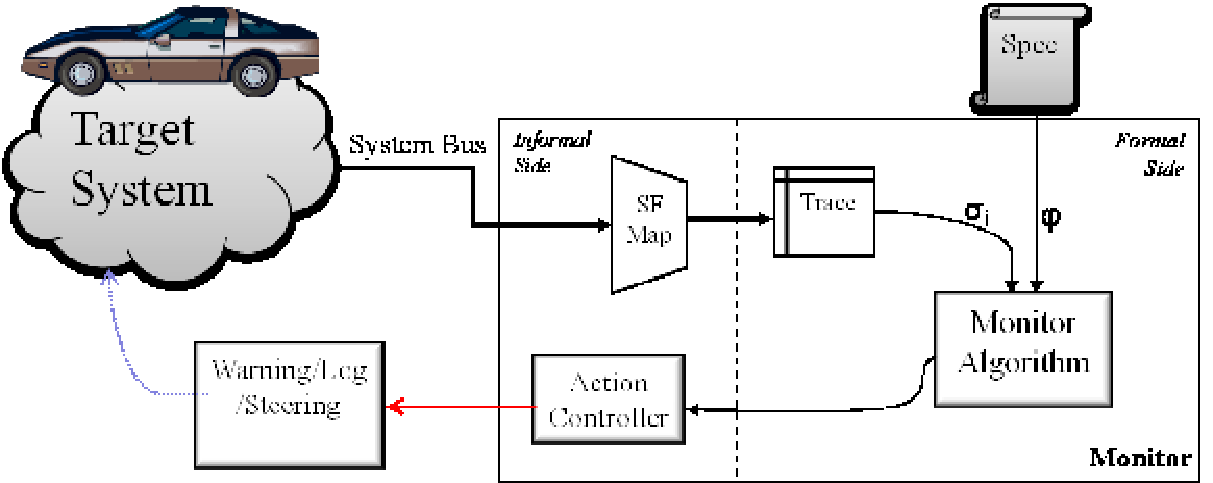
\includegraphics[width=4.5in]{img/mon_arch}
\caption{External monitor architecture outline \label{fig:architecture}}
\end{figure}

This architecture separates the system-independent formal aspects of the monitor from the system-dependent components including the semi-formal interface and system configurations. 
%By utilizing a semi-formal interface, we can separate the formal aspects of the monitor, which are completely independent from the target system, from the more practical pieces: the monitor interfaces and their configurations, which are system dependent. 
This allows us to utilize a core formal monitoring algorithm and framework with any system where an interface map can be used to create a state snapshot. 
Separating the system dependent and system-independent aspects of the monitor also lets the high level system requirements be somewhat abstracted away from the implementation. This means that changes to the target system may only require changes to the interface configuration and not the high level system specification. This is a similar situation to the two-level specifications used in the MaC framework \cite{Kim2004}.

\subsection{System Interface}
Different systems have varying specification needs which can not always be easily met within a formal specification language. In order to provide flexibility to map system state onto the formal specification language (in our case, in propositions) we provide a semi-formal system interface which defines the mapping between the observed system state and the monitored specification. This type of interface is common in monitors for real systems, including MaC's filters \cite{Kim2004} and the AP evaluation filter from \cite{Heffernan2014}.

\subsection{Hybrid Algorithm}
Our eager monitoring algorithm attempts to evaluate specification rules as soon as possible, but this requires checking extra rules


Though early detection of specification violations can be useful, for example to initiate a recovery sooner, performing these eager checks requires more computation.
%
There are situations where eagerly checking a target specification would take too much time to guarantee real-time monitoring correctness. To enable the benefits of eager checking while avoiding the risks of losing real-time correctness, we have implemented a hybrid eager monitoring algorithm which performs non-eager (conservative) checking first and uses any spare time to eagerly check remaining monitor residues.

Under our periodic sampling design, the conservative check is guaranteed to only need to check a single residue for each specification policy in every step (plus updating structures or saving history once per step). 
This conservative check can be done quickly at each period, leaving any extra time until the next check for eager checking. This provides a guarantee that at least the specification is checked within a known delay (i.e., a promptness guarantee) and allows the monitor to eagerly check as much as possible. 
As long as we know that the worst case execution time for message handing, incrementing the structures, and a single residue check is short enough to finish within a monitor period then we are guaranteed at least a conservatively correct and prompt output.

We implemented the hybrid monitoring algorithm in our embedded monitor, which updates the shared monitoring structures and performs a conservative check once every monitoring period, and the uses the idle time between periods to perform eager checking of any remaining unchecked specification properties.
%
Figure \ref{fig:arch:oscope} shows the execution of the embedded monitor instrumented to output the currently executing task to an oscilloscope. This task output was captured using the specification discussed in Section \ref{sec:monspec} plus another 200 time-step \emph{eventually} rule which was never satisfied (so every step the monitor performed all 200 eager checks and could not reduce any remaining formulas. Even with this wasted computation there was still a large portion of idle time -- 23ms of the 25ms loop was spent idle. This shows the eager checking finished reasonably quickly and the monitor could handle much longer formula durations or more complex formulas before the execution time becomes bad enough to not guarantee the monitor finishing all of it's desired eager checking in a single monitoring period. 

\begin{figure}
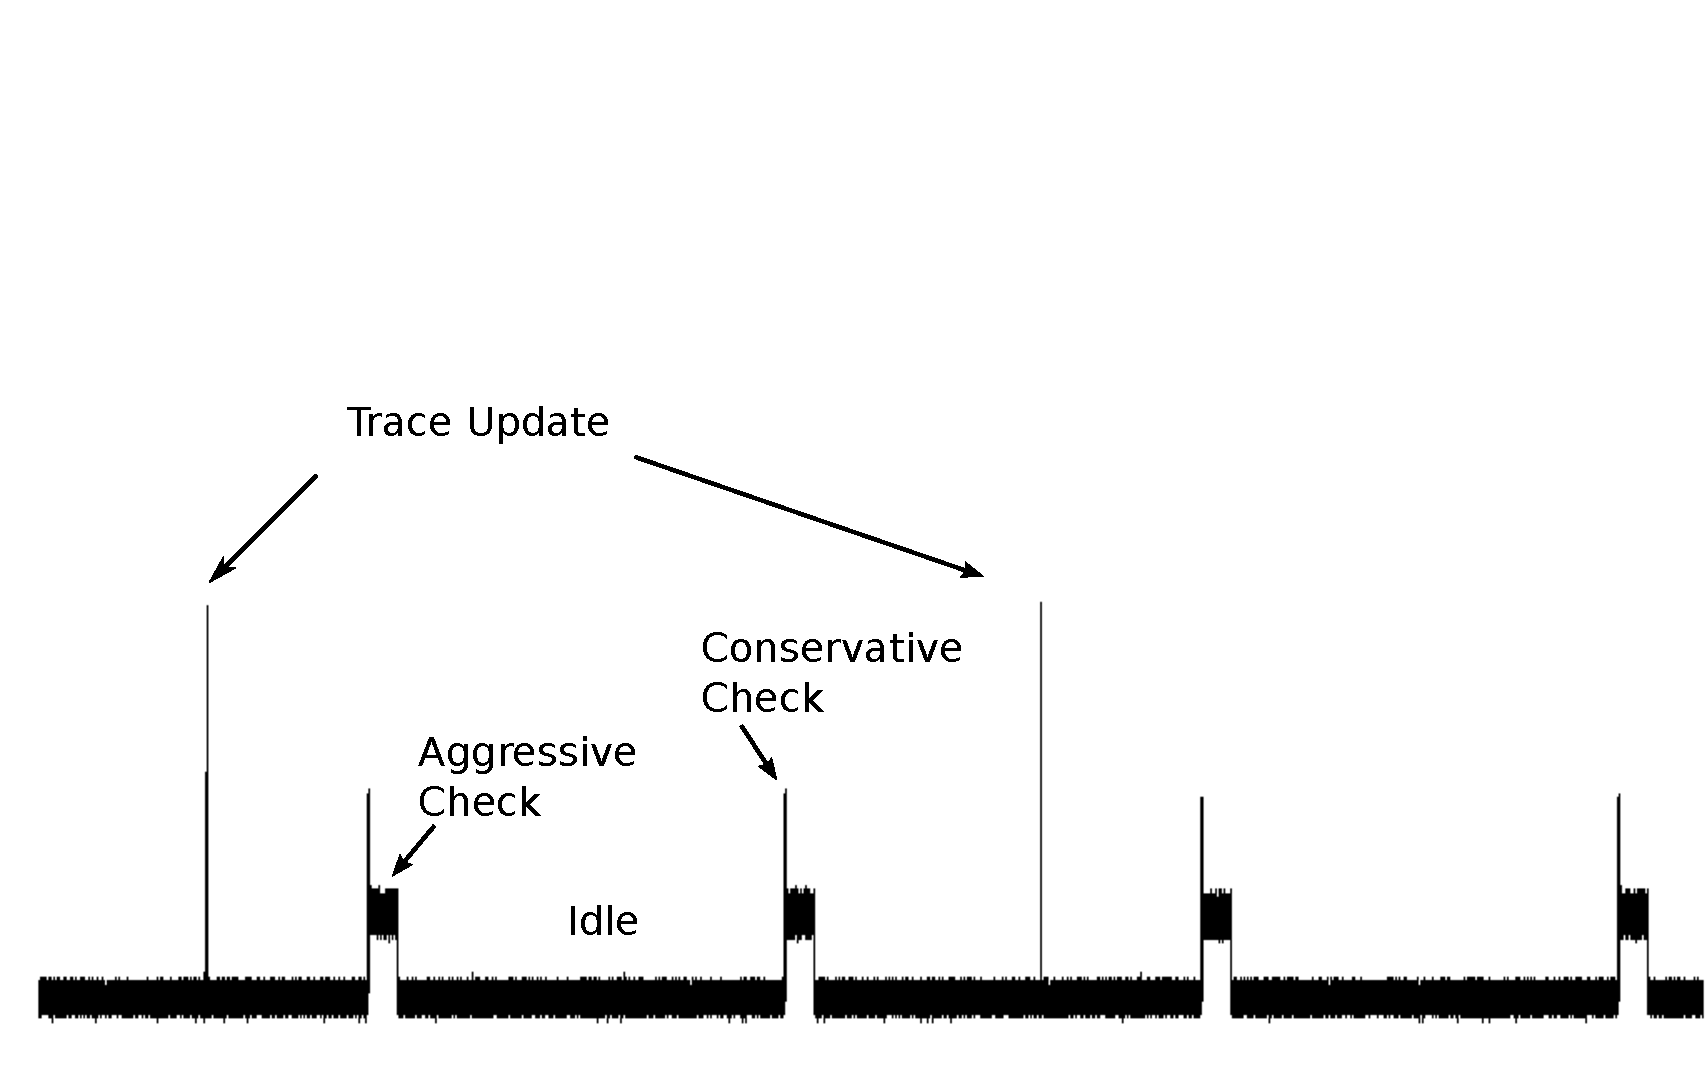
\includegraphics[width=4in]{img/scope_annotated}
\caption{Oscilloscope capture of embedded monitor task execution \label{fig:arch:oscope}}
\end{figure}
